\chapter{Introdução}

O espectro de frequências utilizado para a transmissão de dados é um bem finito. De acordo com estimativas da empresa de redes e telecomunicações Cisco~\cite{ciscoforecast}, estima-se que, em 2018, 20,6 bilhões de dispositivos de rede estarão em funcionamento e o tráfego de dispositivos móveis e sem fio será maior do que o dos dispositivos cabeados. Esse crescimento rápido tem como consequência o congestionamento do meio de transmissão dos dados. Como as frequências são limitadas, torna-se necessária a otimização do uso dos canais.

O uso desses canais é regulamentado por agências governamentais, uma para cada país. No Brasil, existe a Agência Nacional de Telecomunicações (ANATEL),
\abbrev{ANATEL}{Agência Nacional de Telecomunicações}
nos Estados Unidos são regulamentadas pela Federal Communications Commission (FCC),
\abbrev{FCC}{Federal Communications Commission}
na Europa o licenciamento fica a cargo da Electronic Communications Committee (ECC)
\abbrev{ECC}{Electronic Communications Committee}.

As entidades podem comprar o direito de uso de um determinado canal de frequência para uma determinada região. Com isso, tornam-se "Usuários Primários" (UP) \abbrev{UP}{Usuário Primário} daquele canal. Porém, observa-se uma sub-utilização do canal, pois a entidade que o comprou não utiliza em toda a extensão da região. Esses espaços não utilizados, mas com UP, ou seja, com o direito de uso comprado por uma entidade, são chamados de WhiteSpaces (WS).
\abbrev{WS}{WhiteSpaces}
  
Esses WSs poderiam ser utilizados efetivamente por outros dispositivos, porém como não são detentores da licença não podem fazê-lo, gerando um desperdício de canal.

Pela definição do IEEE~\cite{ieee80222}, rádios cognitivos são dispositivos móveis que podem mudar a frequência de transmissão que utilizam dinamicamente. Esses dispositivos se aproveitam do WS utilizando as frequências licenciadas que não estão em uso pelos UPs. Para isso, os dispositivos não licenciados, ou ``Usuários Secundários''(USs)
\abbrev{US}{Usuário Secundário}
devem ser capazes de determinar as frequências disponíveis.

Com isso, um rádio cognitivo é capaz de avaliar o espectro de frequência e escolher um canal livre para transmissão de dados, sendo que esse canal não pode estar sendo usado naquela região pelos UPs, senão geraria interferência. Não é do escopo desse trabalho o modo como o rádio cognitivo realiza a troca de canais. É assumido que os rádios cognitivos modificam sua frequência de transmissão de acordo com o canal que for selecionado.

Caso ocorra uma interferência, ou seja, quando um UP e um US estão transmitindo na mesma frequência, gerando uma superposição das ondas e consequentemente a perda de informação, o rádio cognitivo deve interromper a transmissão imediatamente e buscar outros canais livres.

\begin{figure}[htb]
\centering
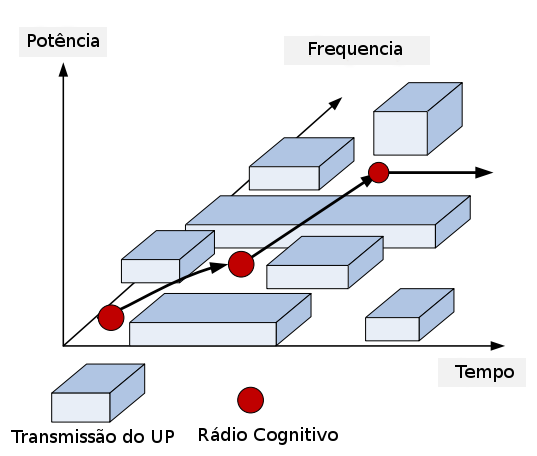
\includegraphics[width=0.8\textwidth]{figs/cr_functioning_over_time}
\caption[Comportamento do rádio cognitivo em função do tempo]
{Comportamento do rádio cognitivo em função do tempo}
\label{fig:funcionamentodoradiocognitivo}
\end{figure} 

Um rádio cognitivo pode utilizar dois modelos diferentes para escolha de um canal livre no espectr. Seu comportamento pode ser observado na figura ~\ref{fig:funcionamentodoradiocognitivo}.

A primeira é pelo sensoriamento. O rádio cognitivo deve possuir um \textit{hardware} específico para ser capaz de analisar as diferentes frequências em utilzação no espectro. Sua implementação é complexa e aumenta o custo de produção do rádio, por conta do \textit{hardware} específico. Os métodos de sensoriamento do espectro não fazem parte do escopo desse trabalho.

A segunda forma é a criação de uma base de dados com a disponibilidade do espectro de frequência em uma dada localização. Com isso, o rádio cognitivo precisa apenas consultar essa base para saber quais canais estão livres naquele momento no seu local. No entanto, para consultar essa base, o rádio precisa estar conectado à rede previamente e então verificar qual canal pode ser utilizado, limitando a sua implementação.

\section{Motivação}

Utilizando o modelo de base de dados, todas as informações são centralizadas e controladas pelas agências reguladoras, o que é uma grande vantagem perante o modelo de sensoriamento, pois caso fosse utilizado, o rádio não teria a necessidade de consultar a base da agência reguladora. Outra grande vantagem é a manutenibilidade. Caso alguma resolução mude, basta aplicar essa regra na base que todos os rádios cognitivos seguirão, já que dependem da resposta da base. Caso fosse via sensoriamento, seria necessário uma reprogramação dos rádios, o que seria custoso e demorado.

Atualmente, os Estados Unidos e Reino Unido já possuem essa base e outros países estão desenvolvendo, como o Canadá.
Também está em fase de desenvolvimento o Protocol to Access White Space database (PAWS)\abbrev{PAWS}{Protocol to Access White Space database}, protocolo para comunicação entre os dispositivos e as bases de WSs~\cite{RFC6953}, pelo Internet Engineering Task Force (IETF)\abbrev{IETF}{Internet Engineering Task Force}.


\section{Objetivo}

A base de dados utilizada foi implementada anteriormente em um trabalho de fim de curso ~\cite{tccmarcelo} e um servidor é responsável pela comunicação com dispositivos que queiram consultar a base. O objetivo desse trabalho foi dar continuidade ao desenvolvimento dessa base, adicionando tabelas para persistência dos dados no banco de dados e um novo modelo de propagação do sinal, que leve em consideração o relevo. Também criou-se um servidor Web para visualização do espectro em um mapa de calor, consulta de canais livres e visualização dos alcances das antenas.

\subsection{Metodologia}

No trabalho realizado foi tentado reproduzir as capacidades de sites já existentes, como o Spectrum Database, do Google~\cite{googlespectrumdatabase}. Para isso, pesquisou-se bibliotecas para exibição de mapas geográficos em páginas Web e exibição de mapas de calor. Em seguida, foi modelado uma aplicação Web que apresenta uma página e permite a interação com a base dados, visualização dos dados e análise do espectro de frequência. Em seguida, foi implementada também a visualização das antenas no Estado do Rio de Janeiro e seus respectivos alcances. Por fim, um novo modelo foi adicionado ao servidor, levando em conta o relevo do Estado do Rio de Janeiro.


